\subsubsection{Graph Viewer}
The Graph Viewer was implemented using ChartActivity and TimelineChart.
ChartActivity is an Activity which holds a GraphicalView (an AchartEngine class
used to encapsulate a chart) and has add and remove buttons on the ActionBar to
edit the products currently displayed. The TimelineChart class is used to build
the dataset, chart and handle changes to the chart as well. The type of chart
currently used is AchartEngine's TimeChart, which is basically a line chart plot
of prices against time. 
\begin{figure}[h!]
\centering
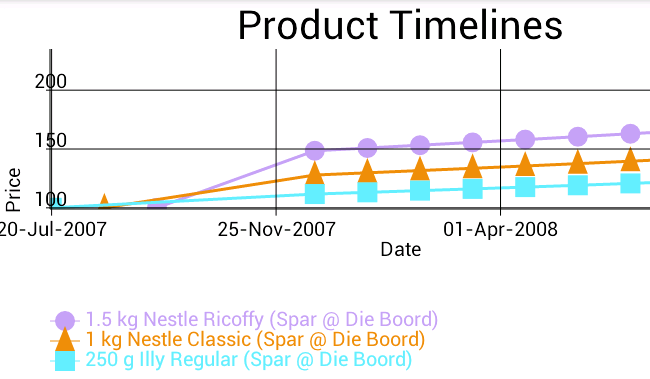
\includegraphics[width=0.5\textwidth]{graph.png}
\caption{Product price histories.}
\end{figure}
